
\documentclass[12pt]{article}
\usepackage[margin=1in]{geometry}
\usepackage[pdftex]{graphicx}
\usepackage{multirow}
\usepackage{setspace}
\usepackage{enumitem}
\pagestyle{plain}
\setlength\parindent{0pt}

\begin{document}

% Course information
\begin{tabular*}{\textwidth}{l @{\extracolsep{\fill}} r}
  & \multirow{3}{*}{
\includegraphics[height=1.0in]{logo.jpg}} \\
  \large Computers in Physics Exps. & \\
  \large Spring Quarter 2019 & \\
  \large Physics 116C & \\
\end{tabular*}
\vspace{10mm}


% Professor information
\begin{tabular}{ l l }
  \multirow{6}{*}{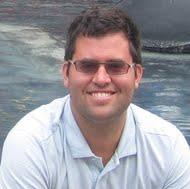
\includegraphics[height=1.25in]{mike.jpg}} & \\
  & \\
  & \large Michael Mulhearn \\
  & \large mulhearn@physics.ucdavis.edu \\
  & \large Physics 317 \\
  & \\
\end{tabular}
\vskip 0.5cm
\noindent
\begin{tabbing}
\hspace*{9em}\= \hspace*{10em} \= \hspace*{6em} \= \kill % set the tabbings
\textbf {Lectures:} \> MWF  1:10-2:00 PM \> 140 Physics \\
%\> \> 152 Roessler \> (F) \\
\hspace*{9em}\= \hspace*{5em} \= \hspace*{8em} \= \kill % set the tabbings
\\
\textbf {Lab:}    \> Section 1: \>  M 4:10-7:00 PM \>152 Roessler \\
                        \> Section 2: \> W 3:10-6:00 PM \> 152 Roessler \\
\\
\hspace*{9em}\= \kill % set the tabbings
\textbf {References:}  \>  {\tt https://www.scipy-lectures.org} \\
\> Online lecture notes on data analysis. \\
\\
\textbf{Office Hours:} \> Monday 2:00-3:30 in Room 317 \\
\textbf{Lab Instructor:} \> Rahim Ullah \\
\textbf{Midterm Exam:} \> May 22, 2019 (during lecture)  \\ 
\textbf{Final Exam:} \> June 13, 2019 at 1:00 PM in Physics 140 \\
\end{tabbing}

\noindent
\textbf {Course Description:}  
Modern experiments rely heavily on microprocessors to acquire and analyze experimental data.  This course uses the Arduino microprocessor as a platform for creating data acquisition systems in different experimental contexts.   We will use Scientific Python for analysis of experimental data.  Topics include statistical distributions, experimental uncertainties, statistical analysis, Fourier analysis, and noise.\\

\noindent
\textbf {Friday Exercises:} 
As much as possible, Friday lectures will be used for in-class exercises using Scientific Python.   Bring a laptop to class on Friday.  If this presents a personal financial hardship, please contact the instructor.  Completed Scipy notebooks should be exported to PDF and submitted to the course website for grading.  \\

\noindent
\textbf{Homework:}  There will be approximately three homework assignments covering the lecture material.\\

\noindent
\textbf {Labs:} 
You are expected to attend every lab session.  The TA will take attendance at the start of each lab. If you arrive late, you should check in with the TA.   Most labs have one or more sign-off points where you are expected to show the TA your setup.  If time permits, the TA may ask a questions of each lab partner.  For example, to describe the purpose of a particular line of code.  When appropriate, you may be assigned a grade for neatness of your experimental setup and/or code.\\

\noindent
\textbf {Lab Safety:} 
You should complete the online course for Electrical Safety at \\
{\tt http://safetyservices.ucdavis.edu/training/electrical-safety}.\\

\noindent
\textbf {Lab Reports:} 
There will be three long lab reports for the Geiger Lab, Johnson Noise Lab, and the Muon Lifetime lab.  The remaining labs include instructions for a report, generally much shorter with fewer requirements.

\begin{samepage}
\vskip 0.5cm
\noindent
\textbf {Course Outline}:
In addition two the listed topic, most weeks we'll need to cover some additional material in lecture to prepare for the upcoming labs.  Labs marked (LW) have a long write-up.  The muon lifetime lab is data analysis only.

\begin{table}[h!]
\begin{tabular}{ lllll }
\hline
\textbf{Week} & \textbf{Dates} & \textbf{Lecture} & \textbf{Lab}  & \textbf{Exercise}\\
\hline
1 & 1,3,5 Apr & Distributions & Intro to Arduino & Plotting \\
\hline
2 & 8,10,12 Apr &  Uncertainties& Geiger Counter (LW) & Histograms \\
\hline
3 & 15,17,19 Apr &  Statistical Analysis & Geiger Counter (cont.)  & \\
\hline
4 & 22,24,26 Apr &  & Arduino Function Generator & \\
% F:  Fourier Analysis
\hline
5 & 29 Apr 1,3 May & & Arduino Digital Scope & Fitting \\
\hline
6 & 6,8,10 May & Fourier Analysis & Arduino Spectrum Analyzer & Muon (LW)\\
\hline
7 & 13,15,17 May & Noise & Johnson Noise (LW) \\
% F: 
\hline
8 & 20,22,24 May & Microprocessors & Johnson Noise (cont.)\\
% F:  LMC Emulation
\hline
9 & (27),29 31 May &  &  No Lab \\
% F: 
\hline
10 &  3,5 Jun &  Review & Arithmetic Logic Unit\\
% F: 
\hline
\end{tabular} 
\end{table}
\end{samepage}
\end{document}

